\section{Results}
After paring down data for a specific building (Packard in this case)
we get a design matrix of 427 observations with a total of 191 detected
access points. We denote $X$ as our design matrix, with each row 
$x_n$ being a vector in $\mathbb{Z}^191$ with each dimension representing
the signal strength of each access point (AP) detected by at least 
one observation.  We also have the labels, $Y$, which represent the 
estimated GPS location given. Each row of $Y$, $y_n$ contains latitude,
longitude, and the error estimate given by the phone.  From here we can actually
generate a likelihood function. The standard equation is:
\begin{equation}
    J(\theta)= \sum_{i=1}^{N} w_i(y_i - \theta^T x_i)^2
\end{equation}
We use the standard weight function, 
\begin{equation} 
    w_i = exp \Bigg( \frac {-\| x_i - x \|_2} {2 \tau^2} \Bigg)
\end{equation}
However, instead of performing a least squares regression, 
we treat each $y_i$ as a guassian RV with mean at it's location, and 
a variance proportional to it's error estimate. We simplify calculations
by converting the PDF of each $y_i$ to be in terms of $r$:
\begin{equation} 
    P_{y_i}(r) \propto exp \Bigg( \frac{\| y - y_i \|^2} {error^2} \Bigg) / error^2
\end{equation}
This yields our location estimate y as:
\begin{equation}
    J(y)= \sum_{i=1}^{N} w_i * P_{y_i}(\|y_i - y\|)
\end{equation}

\begin{figure}
\scalebox{0.5}{
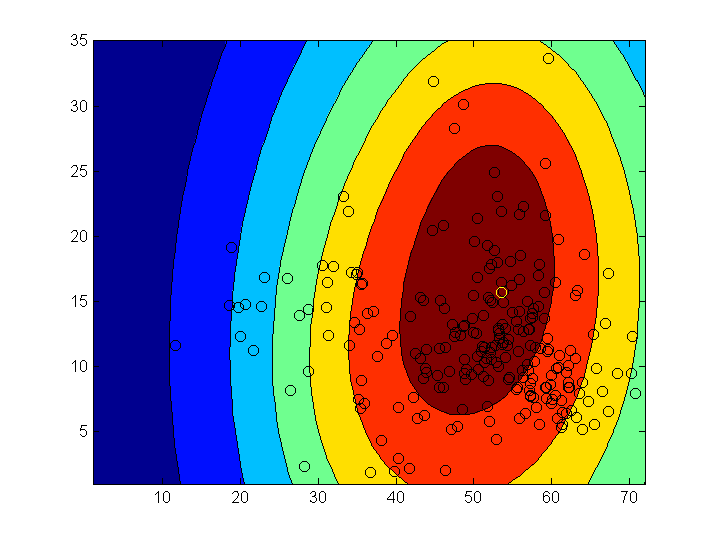
\includegraphics{Contour.png}}
\caption{The original GPS readings are black points. For the selected
observation, shown in yellow, we generated a likelihood function, shown in a contour plot.}
\end{figure}

\begin{figure}
\scalebox{0.5}{
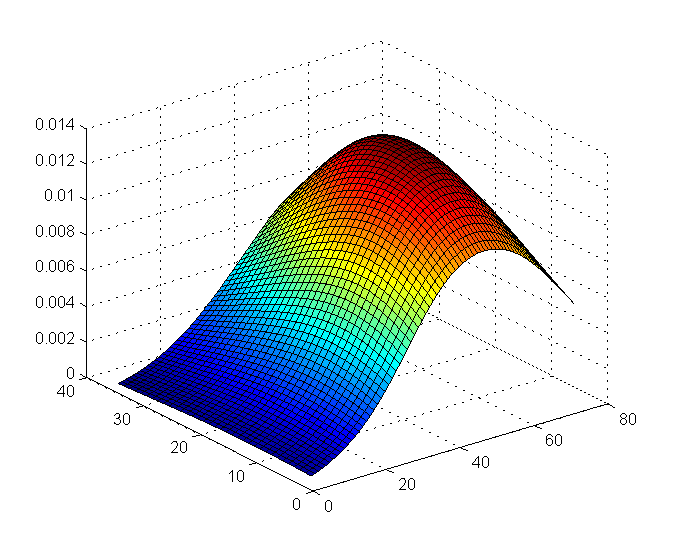
\includegraphics{Surf.png}}
\caption{The likelihood function, plotted over the area of the environment.}
\end{figure}

\begin{figure}
\scalebox{0.5}{
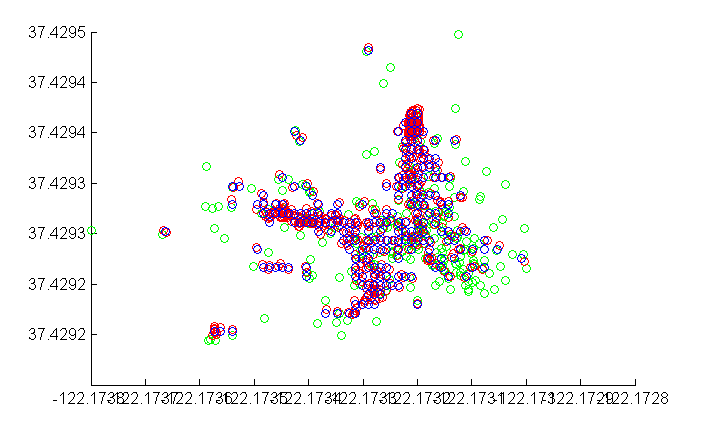
\includegraphics{Plot.png}}
\caption{Figure 3: Maximum likelihood estimates (blue), contrasting with the
original data (green). We added a small noise component (red) to the
blue points because many of the estimates were overlapping.}
\end{figure}

\begin{figure}
\scalebox{0.5}{
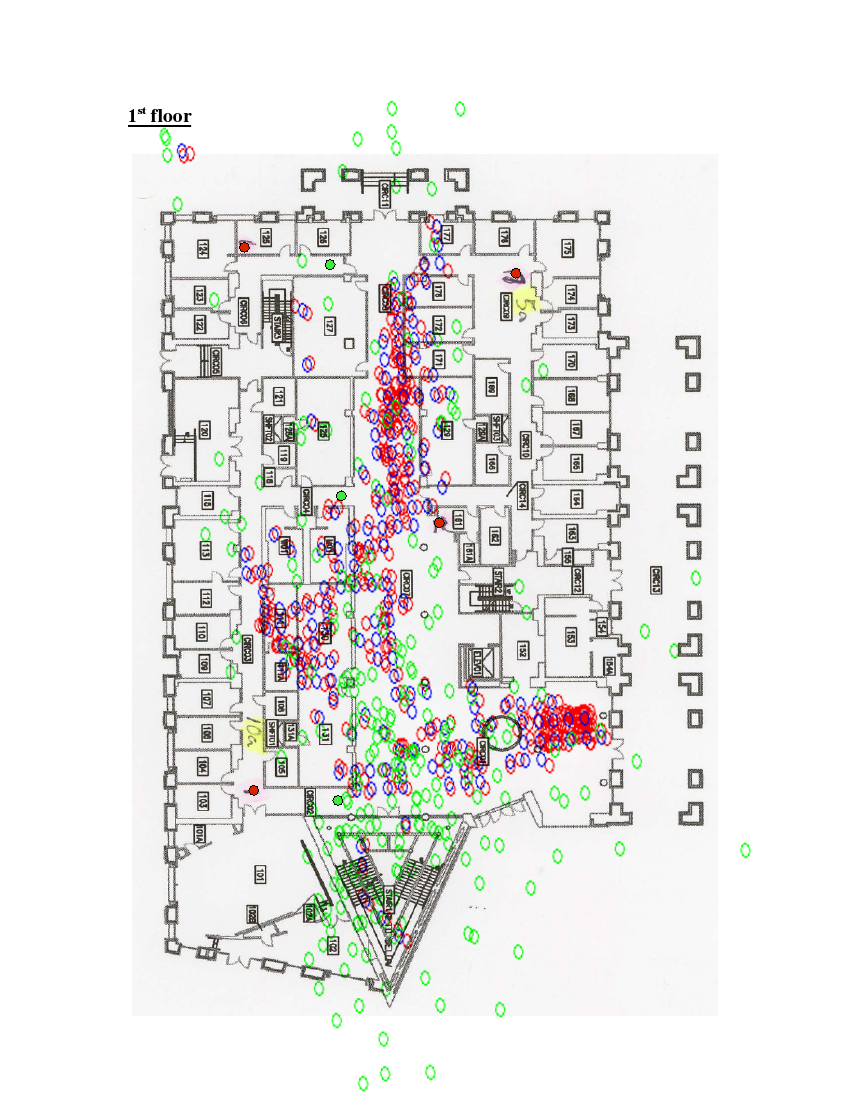
\includegraphics{Overlay.png}}
\caption{The same data points, overlaid on top of Packard's first floor}
\end{figure}

While this function is certainly not convex, we find that in practice, this 
function is well behaved and we can thus easily find maximum estimates of it.
For each observation, we generated a likelihood function using this equation.
We then chose the maximum value over the
distribution to be our MLE for the coordinates of the chosen
observation. Iterating over the entire data set, we generated a rough
plot of the building's layout.
For a data set of 427 observations of 191 access points, our algorithm
had a run time of about 10 to 20 seconds. While this certainly seems slow,
in fact only one observation will have to be run for a given person, which 
means that for a given observation, we can have a computation time of less than a
tenth of a second, an acceptable speed for the given application.
